\pdfminorversion=4
\documentclass[aspectratio=169]{beamer}

\mode<presentation>
{
  \usetheme{default}
  \usecolortheme{default}
  \usefonttheme{default}
  \setbeamertemplate{navigation symbols}{}
  \setbeamertemplate{caption}[numbered]
  \setbeamertemplate{footline}[frame number]  % or "page number"
  \setbeamercolor{frametitle}{fg=white}
  \setbeamercolor{footline}{fg=black}
} 

\usepackage[english]{babel}
\usepackage{inputenc}
\usepackage{tikz}
\usepackage{courier}
\usepackage{array}
\usepackage{bold-extra}
\usepackage{minted}
\usepackage[thicklines]{cancel}
\usepackage{fancyvrb}

\xdefinecolor{dianablue}{rgb}{0.18,0.24,0.31}
\xdefinecolor{darkblue}{rgb}{0.1,0.1,0.7}
\xdefinecolor{darkgreen}{rgb}{0,0.5,0}
\xdefinecolor{darkgrey}{rgb}{0.35,0.35,0.35}
\xdefinecolor{darkorange}{rgb}{0.8,0.5,0}
\xdefinecolor{darkred}{rgb}{0.7,0,0}
\definecolor{darkgreen}{rgb}{0,0.6,0}
\definecolor{mauve}{rgb}{0.58,0,0.82}

\title[2023-05-09-chep23-analysis-of-physicists]{Analysis of physics analysis}
\author{Jim Pivarski}
\institute{Princeton University -- IRIS-HEP}
\date{May 9, 2023}

\usetikzlibrary{shapes.callouts}

\begin{document}

\logo{\pgfputat{\pgfxy(0.11, 7.4)}{\pgfbox[right,base]{\tikz{\filldraw[fill=dianablue, draw=none] (0 cm, 0 cm) rectangle (50 cm, 1 cm);}\mbox{\hspace{-8 cm}
\includegraphics[height=1 cm]{princeton-logo-long.png}\hspace{0.1 cm}\raisebox{0.1 cm}{
\includegraphics[height=0.8 cm]{iris-hep-logo-long.png}}\hspace{0.1 cm}}}}}

\begin{frame}
  \titlepage
\end{frame}

\logo{\pgfputat{\pgfxy(0.11, 7.4)}{\pgfbox[right,base]{\tikz{\filldraw[fill=dianablue, draw=none] (0 cm, 0 cm) rectangle (50 cm, 1 cm);}\mbox{\hspace{-8 cm}
\includegraphics[height=1 cm]{princeton-logo.png}\hspace{0.1 cm}\raisebox{0.1 cm}{
\includegraphics[height=0.8 cm]{iris-hep-logo.png}}\hspace{0.1 cm}}}}}

% Uncomment these lines for an automatically generated outline.
%\begin{frame}{Outline}
%  \tableofcontents
%\end{frame}

%% https://indico.jlab.org/event/459/contributions/11547/

%% Analysis of physics analysis
%%  9 May 2023, 16:00
%%  15m
%%  Marriott Ballroom VI-VII (Norfolk Waterside Marriott)

%% Speaker
%%  Pivarski, Jim (Princeton University)
%% Description
%% Data analysis in particle physics is socially distributed: unlike centrally developed and executed reconstruction pipelines, the analysis work performed after Analysis Object Descriptions (AODs) are made and before the final paper review—which includes particle and event selection, systematic error handling, decay chain reconstruction, histogram aggregation, fitting, statistical models, and machine learning—are often performed “off the GRID.”

%% This presents a challenge for developers of analysis tools, who need to know how their tools are being used in order to focus efforts in development, documentation, and training. The most common methods have traditionally been direct conversations with known users, wide-cast surveys, and download counts, but each of these has its limitations.

%% In this talk, I will discuss the above as well as new methods of analyzing user behavior: collecting issue comments through GitHub and GitLab APIs, statically analyzing code from thousands of git repositories matching search criteria, and web analytics of documentation sites. Applying these methods to the Awkward Array library reveals the most commonly used functions, slice idioms, and data types, as well as what libraries Awkward Array is commonly used with and how data are transferred between them. Finally, I apply these methods to other physics analysis libraries to show the generality of the techniques.

%% Consider for long presentation	No

% START START START START START START START START START START START START START

\begin{frame}{Dark computing}
\vspace{0.25 cm}
\begin{columns}
\column{1.1\linewidth}
\only<1>{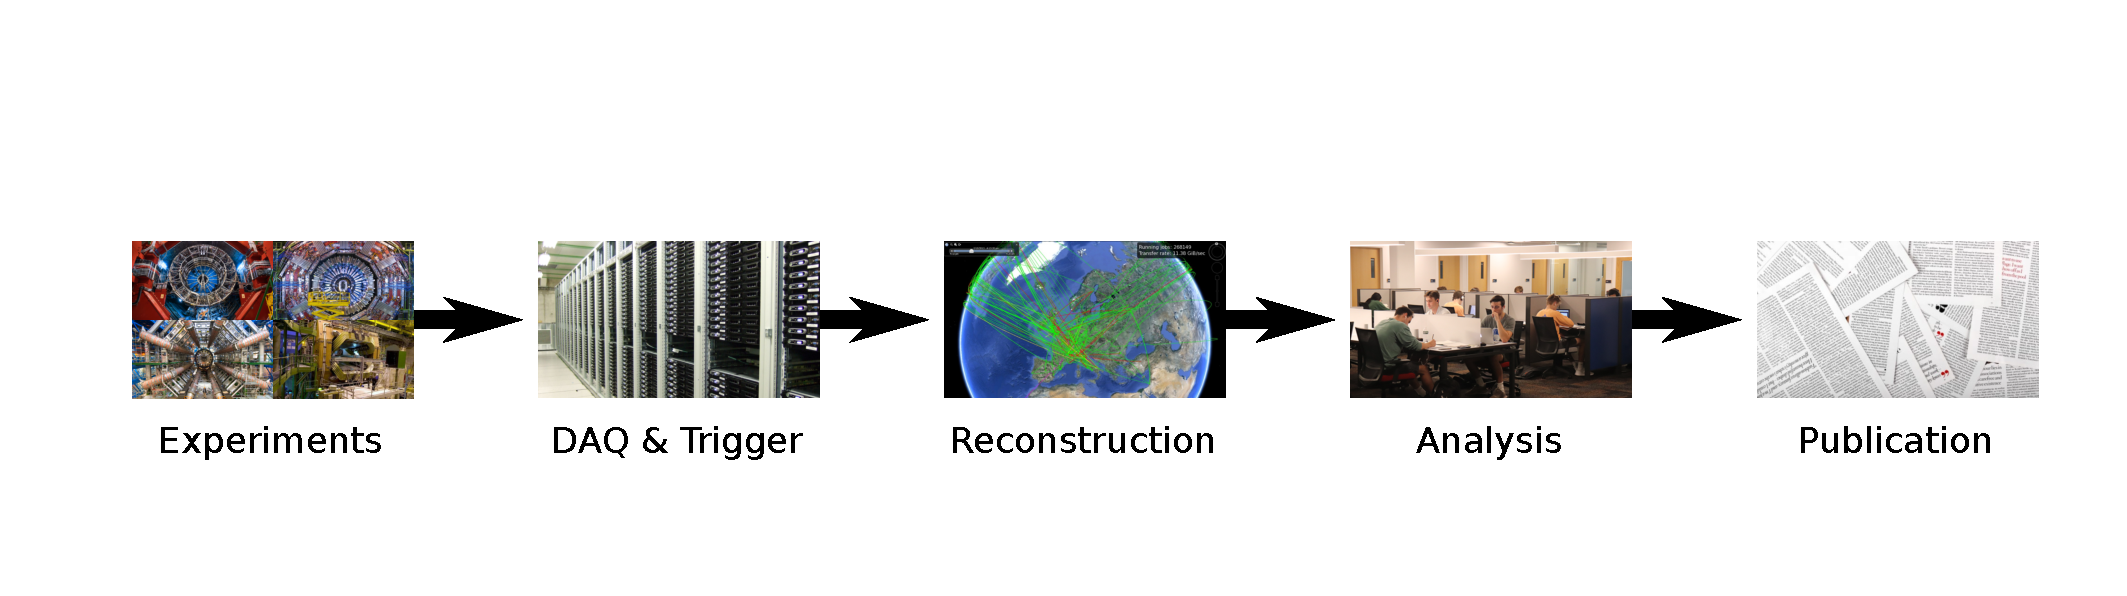
\includegraphics[width=\linewidth]{PLOTS/analysis-chain-0.pdf}}\only<2->{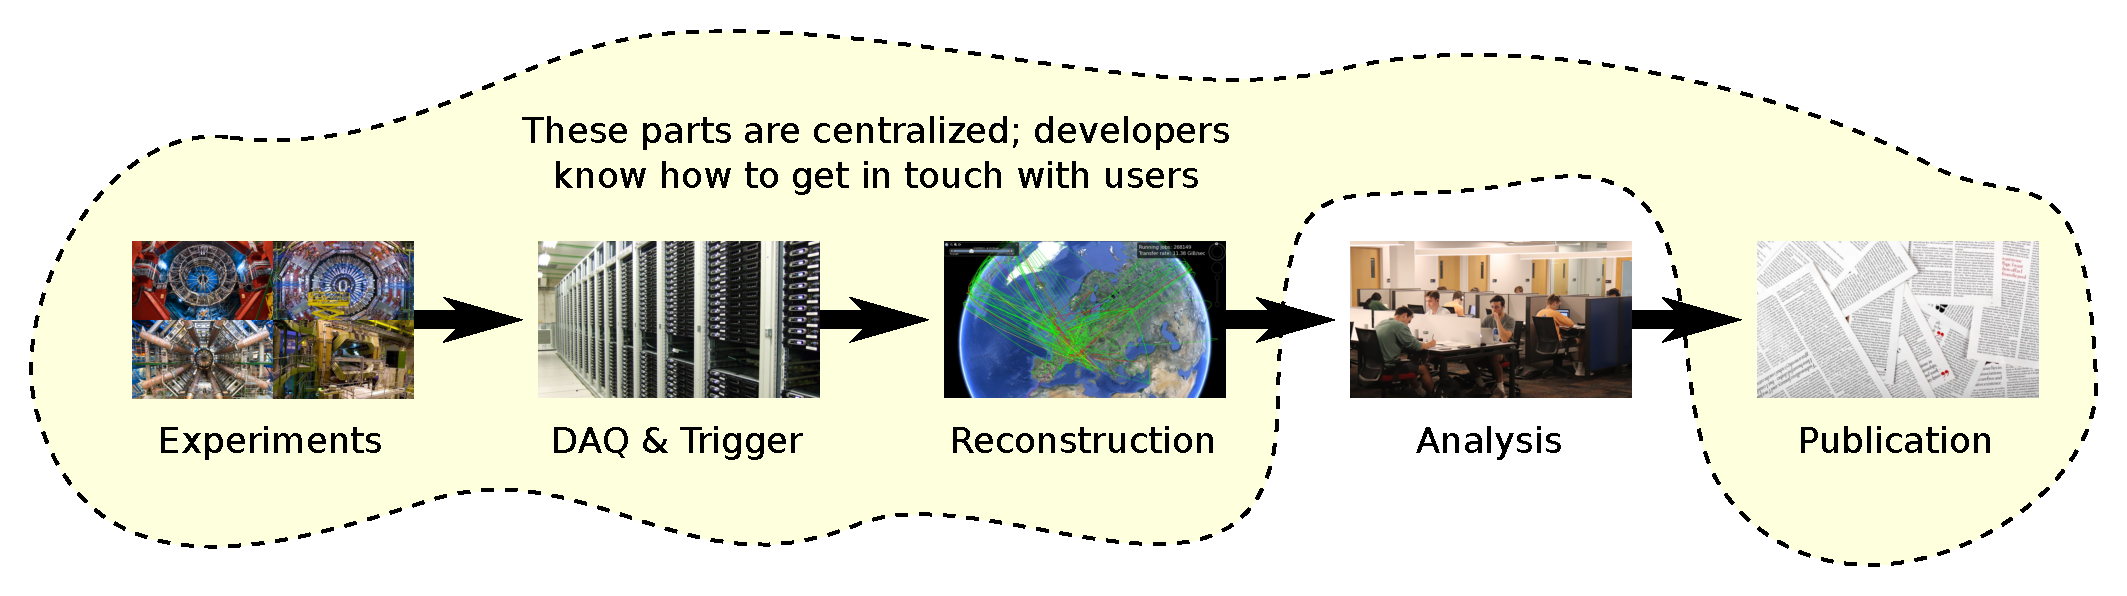
\includegraphics[width=\linewidth]{PLOTS/analysis-chain.pdf}}
\end{columns}

\vspace{0.5 cm}
\begin{itemize}
\item<3-> Good software depends on mutual understanding (between developers and users) of what the software is for and how it's supposed to be used.
\item<4-> The ``analysis'' step is the only one in the pipeline for which we don't even know \underline{\it who} all the users are.
\end{itemize}
\end{frame}

\begin{frame}{We don't do this}
\vspace{1 cm}
\begin{center}
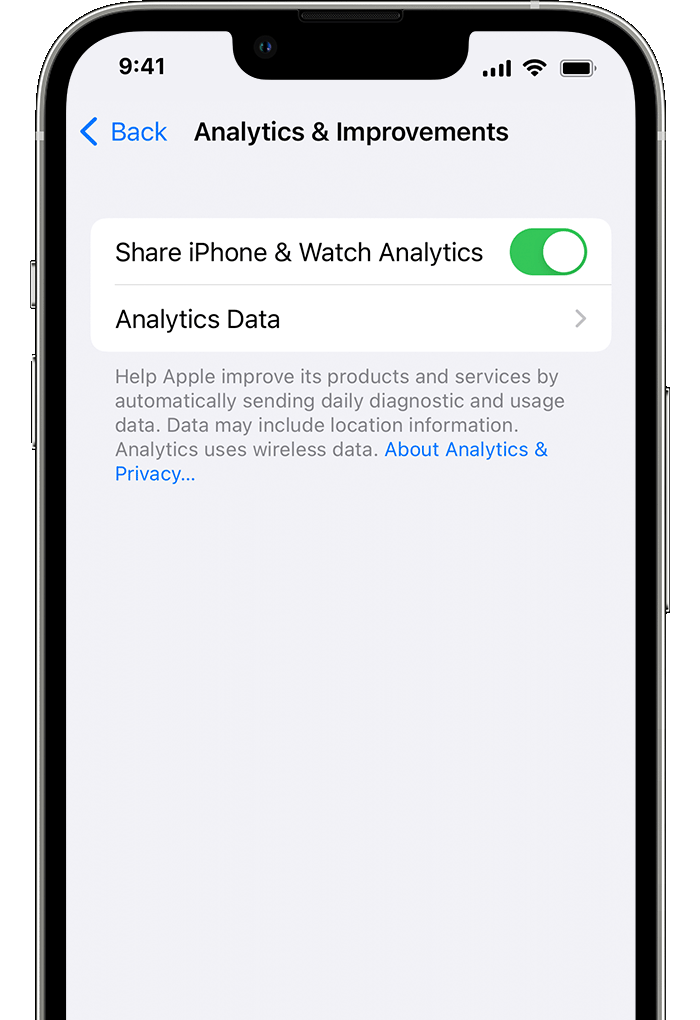
\includegraphics[width=0.5\linewidth]{PLOTS/iphone-send-usage-data.png}
\end{center}
\end{frame}

\begin{frame}{So what can we do instead?}
\vspace{0.35 cm}
\begin{columns}
\column{1.05\linewidth}

\renewcommand{\arraystretch}{0.85}
\begin{tabular}{p{3 cm} p{4.7 cm} p{5.7 cm}}
{\bf Method} & {\bf Good} & {\bf Bad} \\\hline
\uncover<1->{Bug-reports} & \uncover<1->{Resolve immediate needs.} & \uncover<1->{Only hear from proactive people.} \\
\uncover<2->{Surveys} & \uncover<2->{Can directly ask people what they think. Quantitative.} & \uncover<2->{Are the people who didn't fill it out correlated with the questions?} \\
\uncover<3->{Focus groups} & \uncover<3->{As above, but open to free-form response.} & \uncover<3->{Need to generalize from a small group to a large one.} \\
\uncover<4->{Download stats} & \uncover<4->{People vote with their feet. Quantitative.} & \uncover<4->{Skewed by batch jobs. Very coarse-grained info: \underline{\it what} do people like?} \\
\uncover<5->{Textual analysis of CHEP/ACAT} & \uncover<5->{Long-view historical trends.} & \uncover<5->{Only for those who give talks, and what they choose to talk about.} \\
\uncover<6->{Analysis of source code online} & \uncover<6->{Fine-grained, many users, quantitative.} & \uncover<6->{Only public repos, have to identify demographics with some seed: how do you identify ``physicists''?} \\
\end{tabular}
\end{columns}
\end{frame}

\end{document}
